\documentclass{article}
\usepackage[utf8]{inputenc}
\usepackage[T1]{fontenc}
\usepackage{hyperref}
\usepackage{graphicx}
\usepackage{booktabs}
\usepackage{geometry}
\geometry{a4paper, margin=2cm}

\begin{document}

% -------------------------------------------------------------
% APPUNTI 1: SPECTRE, MELTDOWN E FORMAT STRINGS
% -------------------------------------------------------------
\section{Parte 1}
Una \textbf{Race Condition} si verifica quando più processi o thread accedono e manipolano dati condivisi in modo concorrente, e l'esito dell'esecuzione dipende dall'ordine temporale (imprevedibile) degli eventi. Se un programma privilegiato è affetto da questa vulnerabilità, un attaccante può manipolare l'output o il comportamento del sistema.

\subsection{1. TOCTTOU}
\subsubsection{Meccanica dell'Attacco TOCTTOU}
\begin{itemize}
    \item Il programma privilegiato (es. Set-UID root) verifica le autorizzazioni di un file tramite la funzione di sistema \texttt{access()}, basata sull'ID utente reale.
    \item Successivamente, il programma apre il file tramite \texttt{open()}, che utilizza l'ID utente effettivo (in questo caso, root).
    \item L'attaccante sfrutta la finestra temporale che intercorre tra il ``Check'' (\texttt{access}) e lo ``Use'' (\texttt{open}).
    \item Durante questa minuscola finestra, l'attaccante sostituisce il file con un symlink che punta a un file critico di sistema.
\end{itemize}

\begin{figure}[h!]
    \centering
    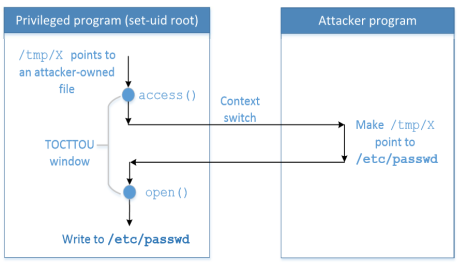
\includegraphics[width=0.5\textwidth]{../picts/tocttou.png}
\end{figure}

\subsubsection{Contromisure per Race Condition}
\begin{itemize}
    \item \textbf{Operazioni Atomiche:} Utilizzare flag specifici come \texttt{O\_CREAT | O\_EXCL} in fase di apertura, che garantiscono la creazione del file solo se questo non esiste, unendo check e use in una singola operazione.
    \item \textbf{Controllo Ripetuto:} Verificare la corrispondenza degli inode tramite \texttt{fstat()} prima e dopo l'apertura del file, abbassando drasticamente le probabilità statistiche di successo dell'attacco.
    \item \textbf{Protezione Symlink (Sticky Symlinks):} Configurare il kernel (\texttt{fs.protected\_symlinks=1}) per impedire di seguire collegamenti simbolici in directory scrivibili da tutti (come \texttt{/tmp}) a meno che il proprietario del symlink non corrisponda al proprietario della directory o del processo.
    \item \textbf{Principio del Minimo Privilegio:} Usare \texttt{seteuid()} per declassare temporaneamente i privilegi di root a quelli dell'utente reale prima di eseguire operazioni su file non fidati.
\end{itemize}

\subsection{2. Dirty COW (Copy-On-Write)}
Dirty COW è una complessa vulnerabilità di Race Condition annidata nei meccanismi di gestione della memoria del kernel Linux, specifica per la funzionalità Copy-On-Write (COW).

\texttt{mmap()}, usata per mappare i file nella memoria virtuale del processo, ha due modalità:
\begin{itemize}
    \item \texttt{MAP\_SHARED} crea una memoria condivisa effettiva tra processi.
    \item \texttt{MAP\_PRIVATE} mappa il file in una memoria privata. Qualsiasi tentativo di scrittura non modificherà il file originale sul disco, ma innescherà il meccanismo Copy-On-Write.
\end{itemize}

Il processo di Copy-On-Write si compone di tre fasi non atomiche:

\begin{figure}[h!]
    \centering
    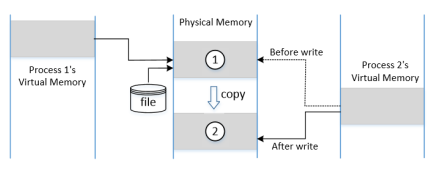
\includegraphics[width=0.5\textwidth]{../picts/dirty_cow.png}
\end{figure}

\begin{enumerate}
    \item Viene creata una copia privata della memoria mappata.
    \item La page table viene aggiornata affinché la memoria virtuale del processo punti alla nuova pagina fisica privata.
    \item Il dato viene scritto nella nuova pagina.
\end{enumerate}

\subsubsection{Meccanica dell'Attacco Dirty COW}
L'attaccante sfrutta la funzione \texttt{madvise()} con il parametro \texttt{MADV\_DONTNEED}, che impone al kernel di scartare la pagina di memoria appena copiata.

L'attaccante lancia due thread concorrenti:
\begin{itemize}
    \item Uno esegue ripetutamente scritture (tramite il filesystem \texttt{/proc/self/mem}).
    \item Uno chiama incessantemente \texttt{madvise()}.
\end{itemize}

Se \texttt{madvise()} viene eseguito esattamente tra il passo 2 e il passo 3 del COW, la tabella delle pagine viene ripristinata per puntare alla memoria fisica originale (di sola lettura). La successiva operazione di scrittura modificherà permanentemente il file originale aggirando i permessi di sicurezza.

\subsection{3. Meltdown e Spectre - Componenti tecniche}
Sia Meltdown che Spectre non derivano da bug del software, ma sfruttano il funzionamento intrinseco e le ottimizzazioni di performance dei processori moderni.

\subsubsection{Fondamenti Architetturali}
\begin{itemize}
    \item \textbf{Out-of-Order Execution:} La CPU esegue le istruzioni non appena le risorse e gli operandi sono disponibili, anticipando il lavoro invece di attendere passivamente. I risultati vengono poi ``ritirati'' (committed) nel corretto ordine logico.
    \item \textbf{Speculative Execution:} Di fronte a un salto condizionale (es. un \texttt{if}), la CPU ``indovina'' quale sarà la strada più probabile da prendere e inizia a eseguirla in anticipo. Se l'ipotesi è errata, i risultati architettonici vengono scartati e lo stato dei registri ripristinato.
    \item \textbf{Caching:} I dati portati in cache durante un'esecuzione speculativa errata \textbf{non} vengono scartati quando lo stato della CPU viene ripristinato.
\end{itemize}

\subsection{4. L'Attacco Meltdown (Rogue Data Cache Load)}
Meltdown rompe il confine di isolamento tra lo user space e il kernel space. Sfrutta una debolezza specifica nella gestione delle eccezioni e dei controlli dei privilegi durante la Out-of-Order Execution, presente in particolar modo nelle architetture Intel.

\subsubsection{4.1 Meccanica di Meltdown}
Il problema fondamentale risiede nel disaccoppiamento temporale tra l'esecuzione di un'istruzione di fetch della memoria e la validazione dei privilegi da parte della Memory Management Unit (MMU).
\begin{itemize}
    \item Quando un'istruzione a livello utente tenta di leggere un indirizzo protetto appartenente al kernel, il controllo fallisce e viene generata un'eccezione (es. un Page Fault \texttt{\#PF}).
    \item Tuttavia, per motivi di latenza, la CPU non attende che l'eccezione venga processata e ritirata (retired) dal ROB prima di forwardare il dato letto dalla memoria (o dalla cache) alle uOps dipendenti successive.
    \item Si crea così una \textbf{transient execution window}: le istruzioni successive usano il dato segreto letto illegittimamente. L'attaccante utilizza questo dato come offset per moltiplicare (es. \texttt{* 4096} per evitare il prefetching) e indicizzare un ``probe array'' nello user space.
    \item Quando l'eccezione viene finalmente sollevata e la pipeline svuotata, il probe array ha già caricato una specifica cache line. Usando tecniche come \textbf{Flush+Reload}, l'attaccante misura i tempi di accesso per individuare quale pagina è in cache, de-offuscando il byte del kernel.
\end{itemize}

\begin{figure}[h!]
    \centering
    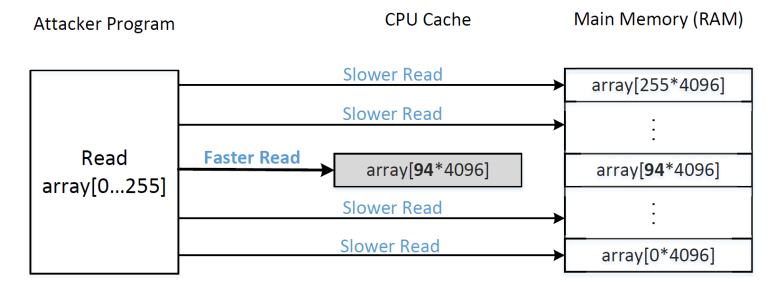
\includegraphics[width=0.5\textwidth]{../picts/meltdown.png}
\end{figure}

\subsubsection{4.2 Mitigazioni per Meltdown}
\begin{itemize}
    \item \textbf{KPTI (Kernel Page-Table Isolation):} Mitigazione software (originariamente KAISER) che separa completamente le page table dello user space da quelle del kernel space. Quando il codice è in user space, la memoria del kernel non è letteralmente mappata (salvo pochissime eccezioni come i gestori di interrupt), bloccando alla radice l'accesso speculativo. Questo introduce un forte overhead a causa dei necessari flush del TLB a ogni context switch, in parte mitigati dall'uso dei \textbf{PCID (Process-Context Identifiers)}.
\end{itemize}

\subsection{5. Spectre}
A differenza di Meltdown, Spectre non viola i confini hardware dei privilegi per leggere la memoria del kernel, ma sfrutta la manipolazione del Branch Predictor per indurre il processo vittima (es. un interprete JavaScript nel browser o un altro processo) a eseguire codice speculativo che rivela i suoi stessi dati segreti.

\begin{figure}[h!]
    \centering
    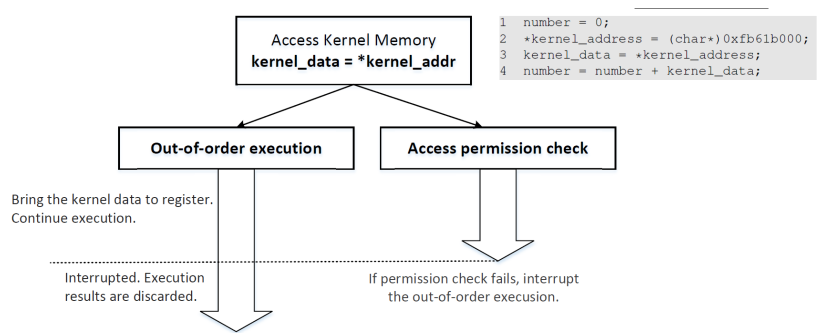
\includegraphics[width=0.5\textwidth]{../picts/spectre.png}
\end{figure}

\subsubsection{5.1 Variante 1: Bounds Check Bypass (CVE-2017-5753)}
Questa variante sfrutta l'addestramento malevolo del predittore dei salti condizionali (Pattern History Table - PHT).
\begin{itemize}
    \item \textbf{Il vettore:} Un classico controllo di sicurezza, come \texttt{if (x < array1\_size) \{ y = array2[array1[x] * 4096]; \}}.
    \item \textbf{Mistraining:} L'attaccante passa valori di \texttt{x} legittimi molteplici volte. Il Branch Predictor impara che il salto condizionale sarà presumibilmente sempre valutato come \emph{True}.
    \item \textbf{L'Exploit:} L'attaccante passa un valore di \texttt{x} fuori limite (out-of-bounds), calcolato affinché \texttt{array1[x]} punti a un dato segreto all'interno della memoria della vittima. La CPU, speculando, ignora il bounds check, carica il byte segreto e lo utilizza come indice per l'operazione su \texttt{array2}. Quando la speculazione viene abortita, la cache L1d conserva la traccia della lettura di \texttt{array2}, esfiltrabile tramite side channel.
    \item \textbf{Mitigazioni:} Mascheramento degli indici (es. clamp/AND logico sull'indice) o l'utilizzo di barriere di serializzazione (es. l'istruzione \texttt{lfence} su architetture x86 o \texttt{csdb} su ARM) poste subito dopo i salti condizionali critici per impedire la speculazione.
\end{itemize}

\subsubsection{5.2 Variante 2: Branch Target Injection (CVE-2017-5715)}
Questa variante avvelena la predizione dei salti indiretti (es. chiamate a puntatori a funzione o metodi virtuali) manipolando il \textbf{Branch Target Buffer (BTB)}.
\begin{itemize}
    \item Poiché il BTB mappa gli indirizzi sorgente alle probabili destinazioni utilizzando spesso solo una parte dei bit dell'indirizzo virtuale, è possibile creare aliasing (collisioni) tra processi diversi.
    \item \textbf{L'Exploit:} L'attaccante esegue salti indiretti nel proprio spazio di indirizzamento progettati per ``inquinare'' il BTB. Quando il processo vittima esegue un normale salto indiretto, il BTB suggerisce speculativamente di saltare a un indirizzo scelto dall'attaccante. Questo target è uno \textbf{Spectre gadget} (simile ai gadget ROP), ovvero codice già presente nella memoria della vittima che accederà al dato segreto e lo inoltrerà al covert channel in cache.
    \item \textbf{Mitigazioni Software (Retpolines):} Introdotta da Google, la \emph{Return Trampoline} sostituisce i salti indiretti con sequenze di \texttt{call} e \texttt{ret}. Questo costringe la CPU a utilizzare il Return Stack Buffer (RSB) invece del BTB per predire la destinazione, intrappolando l'esecuzione speculativa in un loop infinito o innocuo finché la destinazione reale non è risolta.
    \item \textbf{Mitigazioni Hardware:} Aggiornamenti microcodice come \textbf{IBPB} (Indirect Branch Predictor Barrier, che svuota il BTB ai context switch), \textbf{IBRS} (Indirect Branch Restricted Speculation) e \textbf{STIBP} (Single Thread Indirect Branch Predictors).
\end{itemize}

\subsection{1. Introduzione}
Le ``Format String'' (stringhe di formato) sono stringhe di controllo passate alla famiglia di funzioni \texttt{printf()} in C, le quali forniscono un template di output per la funzione. 
Le vulnerabilità legate alle format string, note spesso come \emph{Uncontrolled format string} rientrano nella vasta categoria delle falle da \emph{Improper Input Validation} e \emph{Code Injection}.

Il bug si manifesta quando un utente malintenzionato riesce a controllare direttamente la format string. Questo conferisce poteri enormi all'attaccante, permettendogli nel peggiore dei casi di:
\begin{itemize}
    \item \textbf{Leggere} porzioni arbitrarie di memoria (Memory Read).
    \item \textbf{Scrivere} valori arbitrari in locazioni di memoria scelte (Memory Write).
    \item \textbf{Aggirare} meccanismi di protezione come gli \emph{stack canary}, potendo leggerli dalla memoria o sovrascrivendo direttamente un indirizzo di ritorno senza alterarli.
\end{itemize}

\subsection{2. L'Origine del Bug (Funzioni Variadiche)}
L'anomalia nasce dalle convenzioni del linguaggio C per l'implementazione delle funzioni variadiche (dichiarate terminando l'elenco degli argomenti con i puntini di sospensione \texttt{...}, come in \texttt{int printf(const char *fmt, ...);}). 

Poiché il C non esegue controlli rigorosi sui tipi a runtime per queste specifiche funzioni (mancanza di \emph{type-safety}), il compilatore non verifica il numero né il tipo degli argomenti effettivamente passati.
\begin{itemize}
    \item \textbf{Comportamento normale:} In una chiamata legittima, \texttt{printf()} incontra un carattere di formato (es. \texttt{\%d}) e legge l'argomento successivo dallo stack (sistemi 32-bit) o dai registri/stack (sistemi 64-bit), supponendo che il programmatore lo abbia fornito correttamente.
    \item \textbf{Il vettore di attacco:} Se utilizzata \texttt{printf(buf);} al posto della forma sicura \texttt{printf("\%s", buf);}, \texttt{buf} è esposto all'input utente e la funzione interpreterà ogni \texttt{\%} contenuto all'interno di \texttt{buf} come uno specificatore di formato. Questo costringerà la funzione a estrarre valori dalle locazioni di memoria adiacenti, anche se nessun argomento aggiuntivo era stato originariamente passato.
\end{itemize}

\subsection{3. Tecniche di Exploitation}
\subsubsection{3.1 Letture dello Stack (Stack Reads)}
Il metodo più immediato per è far trapelare informazioni dallo stack:
\begin{itemize}
    \item \textbf{Sistemi 32-bit:} L'invio di una sequenza di \texttt{\%x} forza \texttt{printf()} a stampare i valori esadecimali in successione scendendo nello stack (4 byte alla volta).
    \item \textbf{Sistemi 64-bit:} I primi cinque \texttt{\%lx} rivelano il contenuto dei registri correnti (\texttt{rsi}, \texttt{rdx}, \texttt{rcx}, \texttt{r8}, \texttt{r9}). Dal sesto specificatore in poi, si innesca la lettura delle linee dello stack (8 byte alla volta).
    \item \textbf{Limitazioni:} Se il buffer vulnerabile è di dimensione limitata \texttt{s}, l'attaccante può avanzare al massimo di \texttt{s/2} righe di stack. Potrebbe non essere uno spazio sufficiente per intercettare il canary.
\end{itemize}

\subsubsection{3.2 Accesso Casuale agli Argomenti}
Sfruttando la sintassi \texttt{\%n\$d} (dove \emph{n} indica la posizione dell'argomento), si istruisce la funzione a saltare direttamente all'argomento desiderato.
\begin{itemize}
    \item In passato (e in librerie come \texttt{musl}), questo aggirava completamente i limiti spaziali del buffer.
    \item Secondo lo standard attuale, implementato rigorosamente nelle versioni moderne di \texttt{glibc}, \textbf{non sono ammessi gap}. La funzione deve conoscere la dimensione degli \texttt{n-1} argomenti precedenti prima di saltare all'n-esimo. Di conseguenza, l'accesso casuale non è più una garanzia per raggiungere profondità arbitrarie nello stack.
\end{itemize}

\subsubsection{3.3 Letture Arbitrarie in Memoria (Arbitrary Memory Reads)}
Per leggere un indirizzo specifico, si utilizza lo specificatore \texttt{\%s}, che stampa i caratteri a partire dall'indirizzo fornito fino al primo \emph{null byte} (\texttt{\textbackslash x00}).
\begin{itemize}
    \item Se la format string è anch'essa salvata nello stack, l'attaccante può inserire l'indirizzo esatto che desidera leggere all'interno della stringa stessa. Tramite modificatori (come \texttt{\%c}) spingerà in avanti l'\emph{argument pointer} fino a farlo coincidere con l'indirizzo malevolo memorizzato nel payload.
    \item \emph{Nota operativa:} È necessario calcolare un corretto allineamento della memoria (padding). Inoltre, gli indirizzi contenenti byte nulli vanno posizionati alla fine della stringa di formato, affinché non interrompano in anticipo la lettura di \texttt{printf()}.
\end{itemize}

\subsubsection{3.4 Scritture Arbitrarie in Memoria (Arbitrary Memory Writes)}
L'apice dell'attacco avviene con lo specificatore direzionale \texttt{\%n}. Questo operatore poco noto non stampa nulla a schermo, ma \textbf{scrive} all'indirizzo di memoria puntato l'esatto numero di byte emessi dalla funzione fino a quel momento.
\begin{itemize}
    \item Controllando i byte in output (usando costrutti come \texttt{\%mc} per emettere \texttt{m} byte), un attaccante controlla il valore scritto in memoria.
    \item Poiché generare milioni o miliardi di byte a schermo per scrivere un indirizzo di ritorno intero comporterebbe il blocco o il crash del processo, la tecnica fa largo impiego di troncamenti. Operatori come \texttt{\%hn} (2 byte) e \texttt{\%hhn} (1 byte) permettono di comporre il valore sovrascrivendo l'indirizzo un singolo byte alla volta, azzerando quasi del tutto i contatori in eccesso tramite somme sequenziali del buffer.
\end{itemize}

\textbf{Struttura base di un Payload di sovrascrittura (Tabella Ricostruita):}
\begin{verbatim}
AAAA \x04\x03\x02\x01 BBBB \x05\x03\x02\x01
CCC  \x06\x03\x02\x01 DDD  \x07\x03\x02\x01
\end{verbatim}
\emph{(Le sezioni alfabetiche fungono da pad o dummy arguments per l'allineamento con le sequenze in esadecimale che puntano agli indirizzi contigui in cui scrivere, sfruttando poi vari \texttt{\%hhn} nel resto della payload string per sovrascrivere byte per byte l'indirizzo \texttt{0x01020304}).}

\subsection{4. Mitigazioni a livello di Sistema e Compilatore}
Per arginare l'efficacia di questi vettori, le librerie come \texttt{glibc} e i compilatori come \texttt{gcc} integrano contromisure pesanti:
\begin{enumerate}
    \item \textbf{Macro \texttt{\_FORTIFY\_SOURCE}}: Quando abilitata (sia con valore 1 che con controlli più stretti a valore 2, e in concomitanza con opzioni di ottimizzazione \texttt{-O}), innesca difese critiche a run-time. Ad esempio, il processo viene istantaneamente ucciso (abort) se si invoca l'operatore \texttt{\%n} su una porzione di memoria marcata come scrivibile, oppure se si usa una stringa ad accesso casuale \texttt{\%n\$} omettendo gli argomenti intermedi.
    \item \textbf{\texttt{Wformat-security}}: Un'opzione di compilazione (generalmente integrata nel gruppo \texttt{-Wall}) che forza \texttt{gcc} a emettere messaggi d'errore o avvisi qualora il codice usi la famiglia di funzioni in modo improprio (come usare \texttt{printf(variabile)} senza un vero specificatore esplicito inserito dal programmatore).
\end{enumerate}


% -------------------------------------------------------------
% APPUNTI 2: DNS
% -------------------------------------------------------------
\section{Vulnerabilità DNS}

\subsection{1. Architettura e Spazio dei Nomi DNS}
Il Domain Name System (DNS) è un servizio gerarchico progettato per associare nomi di dominio ad indirizzi IP numerici.

Il sistema si basa su un \textbf{Hierarchical Name Space} organizzato in questo modo:
\begin{itemize}
    \item \textbf{Root Name Servers:} 13 server principali (identificati dalle lettere da A a M) replicati globalmente in oltre 247 istanze tramite anycast.
    \item \textbf{Top-Level Domain (TLD) Servers:} Responsabili per i domini di primo livello generici (\texttt{.com}, \texttt{.org}, \texttt{.net}) e nazionali (\texttt{.it}, \texttt{.uk}).
    \item \textbf{Authoritative Name Servers:} Server che contengono i record DNS definitivi e ufficiali per una specifica organizzazione o dominio (es. server di università o grandi aziende).
    \item \textbf{Local Name Resolvers:} I server contattati inizialmente dai client (spesso forniti dall'ISP) che si occupano di interrogare l'infrastruttura per conto dell'utente quando non conoscono un nome.
\end{itemize}

\begin{figure}[h!]
    \centering
    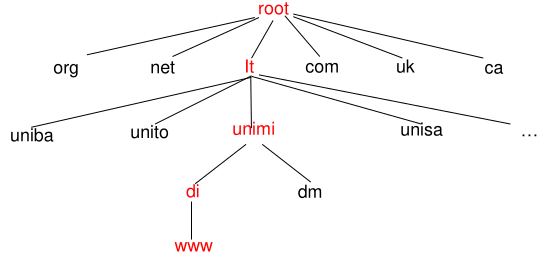
\includegraphics[width=0.5\textwidth]{../picts/dns-hier.png}
\end{figure}

\subsection{2. Zone e Tipi di Record}
Una zona DNS è una collezione di coppie hostname/IP gestite congiuntamente da un Authoritative Nameserver.

I dati all'interno del DNS sono memorizzati in \textbf{Resource Records} (RR) che contengono i campi:
\begin{itemize}
    \item Name
    \item Value
    \item TTL (Time To Live)
    \item Type
\end{itemize}

I tipi principali sono:

\begin{table}[h!]
\centering
\begin{tabular}{ll}
\toprule
\textbf{Tipo Record} & \textbf{Descrizione} \\
\midrule
\texttt{A} & Address record (contiene un indirizzo IPv4) \\
\texttt{NS} & Name Server (punta al server autoritativo per una zona) \\
\texttt{MX} & Mail eXchanger (indica il server responsabile per la posta elettronica) \\
\texttt{CNAME} & Canonical Name (crea un alias, un ``link'' a un altro nome) \\
\texttt{SOA} & Start of Authority (contiene i parametri globali della zona e i contatti dell'amministratore) \\
\texttt{TXT} & Generic text (usato spesso per configurazioni di sicurezza e chiavi pubbliche come DKIM o SPF) \\
\bottomrule
\end{tabular}
\end{table}

\subsection{3. Il Processo di Risoluzione dei Nomi}
La risoluzione si divide in due modalità principali:
\begin{itemize}
    \item \textbf{Recursive Query:} Il server si fa carico dell'intera risoluzione e restituisce al client direttamente la risposta finale (usata tipicamente dai resolver locali degli ISP).
    \item \textbf{Iterative Query:} Il server restituisce una risposta se la conosce, oppure un riferimento (referral) al prossimo server da interrogare (usata nelle comunicazioni tra server DNS).
\end{itemize}

\textbf{Esempio pratico di Lookup (Ricorsivo/Iterativo):}
\begin{enumerate}
    \item Il PC dell'utente interroga il Nameserver locale (ricorsivo) per \texttt{www.unixwiz.net}.
    \item Non avendo il dato in cache, il Nameserver locale interroga uno dei Root Server.
    \item Il Root Server non conosce il dominio finale ma restituisce un \emph{referral} per i server del TLD \texttt{.net}.
    \item Il Nameserver locale interroga il TLD \texttt{.net}, che restituisce a sua volta i record \emph{glue} per gli Authoritative Server di \texttt{unixwiz.net}.
    \item Il Nameserver locale interroga l'Authoritative Server (\texttt{ns.unixwiz.net}) ricevendo il record A (risposta Autorevole).
    \item La risposta viene passata al PC dell'utente e inserita in cache.
\end{enumerate}

\begin{figure}[h!]
    \centering
    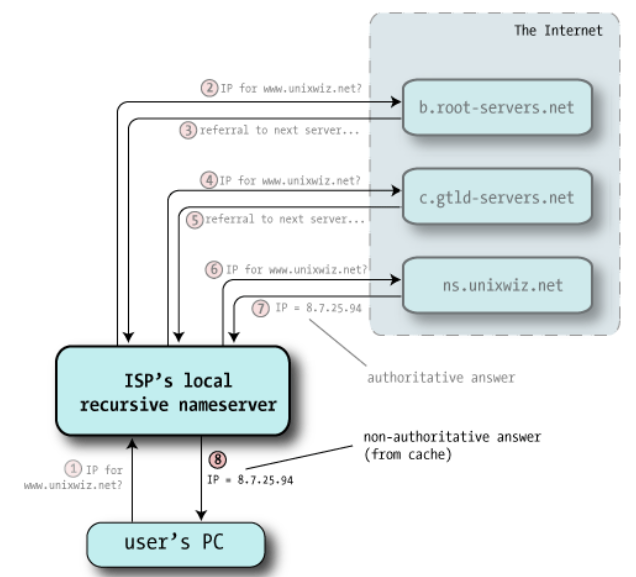
\includegraphics[width=0.5\textwidth]{../picts/dns-res.png}
\end{figure}

\textbf{Risoluzione Inversa:} Il DNS mappa anche gli IP in nomi di host usando l'ordine inverso dei byte dell'IP sotto lo speciale dominio di primo livello \texttt{in-addr.arpa}.

\subsection{4. Pacchetti e Messaggi DNS}
Il DNS utilizza nativamente la porta 53/UDP (e TCP in casi specifici come risposte grandi o zone transfer). I pacchetti hanno una struttura fissa divisa in 5 sezioni:

\begin{table}[h!]
\centering
\begin{tabular}{ll}
\toprule
\textbf{Sezione} & \textbf{Descrizione} \\
\midrule
\textbf{Header} & Contiene il \emph{Query ID} (TXID - fondamentale per accoppiare query e risposte) a 16 bit, e i flag operativi \\
\textbf{Question} & La query effettiva \\
\textbf{Answer} & I Resource Record della risposta \\
\textbf{Authority} & I record SOA o NS rilevanti per la delega \\
\textbf{Additional} & Informazioni extra, spesso ``Glue records'' (gli IP dei nameserver citati in Authority) \\
\bottomrule
\end{tabular}
\end{table}

\begin{figure}[h!]
    \centering
    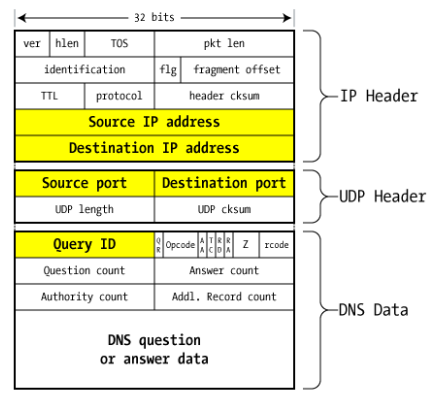
\includegraphics[width=0.5\textwidth]{../picts/dns-packet.png}
\end{figure}

Flags:
\begin{itemize}
    \item \texttt{QR} (Query / Response) 0: query, 1 response
    \item \texttt{Opcode}: 0 for a standard query
    \item \texttt{AA}: Authoritative Answer
    \item \texttt{RD}: Recursion Desired
    \item \texttt{RA}: Recursion Available
    \item \texttt{Z}: reserved must be zero
    \item \texttt{rcode}: success or failure
\end{itemize}

\subsection{5. Vulnerabilità: Cache Poisoning (Avvelenamento della Cache)}
L'obiettivo di un attacco di poisoning è inserire falsi record IP nella cache di un nameserver ricorsivo vittima, dirottando così tutti i suoi utenti verso un server controllato dall'attaccante.

Affinché un DNS accetti una risposta, l'attaccante deve forgiare un pacchetto in cui:
\begin{itemize}
    \item Corrisponda la porta UDP
    \item La ``Question'' corrisponda a quella in attesa
    \item Il Query ID corrisponda alla query in corso
    \item Si rispetti il ``Bailiwick checking'' (il server risponde solo per domini di sua competenza)
\end{itemize}

Il problema con questa versione banale è la dimensione della finestra di attacco: una volta ricevuta risposta l'attaccante deve attendere la scadenza del TTL, diventa quindi molto improbabile indovinare il Query ID.

\subsubsection{Attacco Kaminsky}
Nelle vecchie implementazioni, il Query ID era facilmente predicibile (incrementale), rendendo questo attacco molto più semplice.

\begin{enumerate}
    \item Invece di aspettare che scada il TTL per \texttt{www.banca.com}, l'attaccante invia query per sottodomini inesistenti (es. \texttt{1234.banca.com}, \texttt{1235.banca.com}) forzando il resolver della vittima a inoltrare costantemente richieste ai Root/TLD.
    \item Nel frattempo, l'attaccante inonda il resolver di risposte contraffatte per \texttt{1234.banca.com}, tentando di indovinare il Query ID corretto.
    \item La risposta contraffatta non si limita a risolvere \texttt{1234.banca.com}, ma include nella sezione \emph{Authority} e \emph{Additional} (Glue Records) falsi record che delegano l'intera zona \texttt{banca.com} ai name server dell'attaccante.
    \item Indovinando un solo pacchetto su migliaia (favorito dalla natura stateless di UDP e dal fatto che forzare query genera continue finestre temporali di vulnerabilità), l'attaccante acquisisce il controllo dell'intera risoluzione di zona, dirottando web e email.
\end{enumerate}

\textbf{Difese:} Randomizzazione del Source Port e del Query ID. Usando entrambe le tecniche, lo spazio delle possibilità sale a circa 134 milioni, rendendo il brute-force impercorribile in tempi brevi.

\begin{figure}[h!]
    \centering
    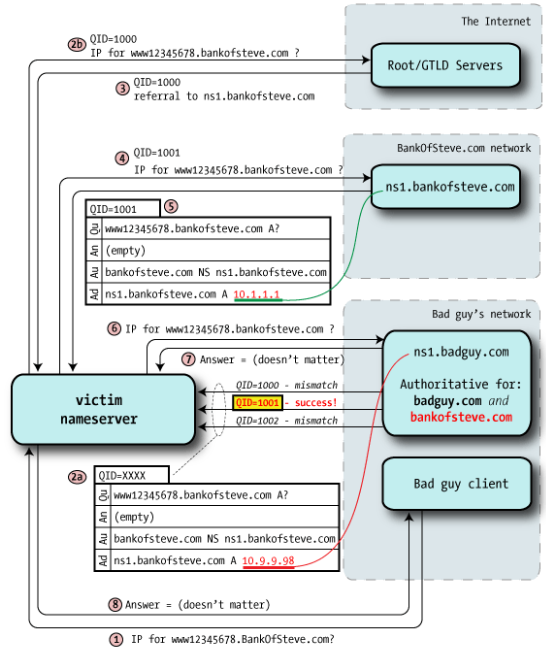
\includegraphics[width=0.5\textwidth]{../picts/kaminsky.png}
\end{figure}

\subsection{6. Attacchi Denial of Service (DoS) e Amplification}
Il DNS è spesso sfruttato come arma o bersaglio di DoS:
\begin{itemize}
    \item \textbf{``Exploit to Fail'':} Sfrutta bug nel parser DNS (es. BIND) inviando pacchetti malformati che mandano in crash il demone (CVE-2002-0400).
    \item \textbf{``Exploit to Own'':} Buffer overflow mirato per eseguire codice remoto e ottenere privilegi di root (VU\#844360).
    \item \textbf{Reflection \& Amplification Attack:} L'attaccante forgia query DNS spoofando l'IP sorgente (mettendo l'IP della vittima). Manda le query a recursor aperti (``Open Resolvers'') su Internet. La query è molto piccola (pochi byte), ma richiede una risposta volontariamente gigantesca (``LARGE DNS Response'' come record ANY o DNSSEC). I server riflettono queste risposte enormi sulla vittima, amplificando drasticamente l'attacco ed esaurendone la banda.
    \item \textbf{NXDOMAIN Cache Exhaustion:} Si inonda il resolver con richieste di domini inesistenti per riempirgli la cache ed esaurire le risorse.
\end{itemize}

\subsection{7. Pharming e DNS Rebinding}
Il Pharming punta a dirottare gli utenti modificando il file hosts del client o compromettendo i router locali.

\subsubsection{DNS rebinding}
Una sofisticata elusione della ``Same Origin Policy'' (SOP) dei browser:
\begin{enumerate}
    \item L'attaccante registra un dominio (\texttt{attacker.com}) e imposta un TTL bassissimo (es. 0 o 60 secondi) sul record A puntando al proprio IP pubblico.
    \item La vittima visita il sito. Il browser risolve il nome nell'IP pubblico dell'attaccante e scarica un payload (JavaScript, Applet).
    \item Il payload attende la scadenza del TTL.
    \item A TTL scaduto, l'Authoritative server dell'attaccante fa un \emph{rebind}: risponde alle nuove query DNS puntando il nome \texttt{attacker.com} non più all'IP dell'attaccante, ma a un IP \emph{interno} alla LAN della vittima.
    \item Il browser, basandosi sul fatto che il ``nome a dominio'' non è cambiato (è sempre \texttt{attacker.com}), crede di rispettare la Same Origin Policy e permette al payload di interagire liberamente con il dispositivo della rete interna e leggerne i dati.
\end{enumerate}

\textbf{Mitigazioni}: è un tipo di attacco scomodo da mitigare, protezioni come DNS Pinning nei browser tendono ad interagire male anche con siti genuini, la soluzione più pratica è un blocco a livello firewall che impedisce di risolvere nomi esterni ad indirizzi interni.

\begin{figure}[h!]
    \centering
    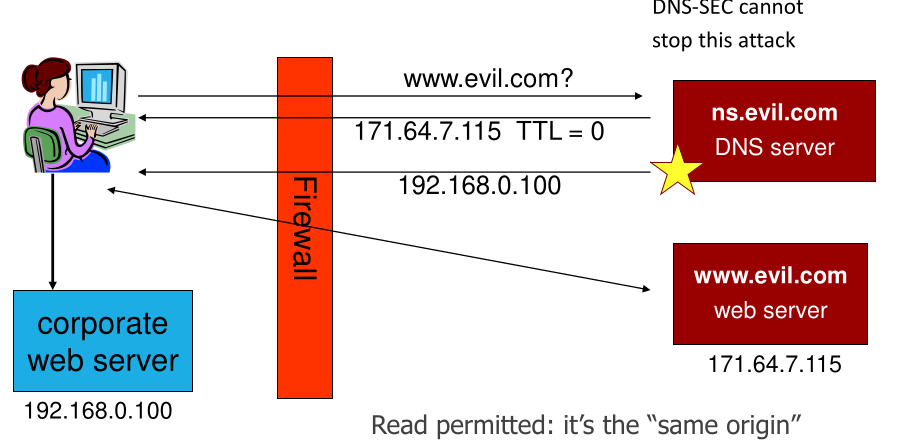
\includegraphics[width=0.5\textwidth]{../picts/dns-rebind.png}
\end{figure}

\subsection{8. DNSSEC: Sicurezza Crittografica}
Progettato dall'IETF per fornire Autenticazione dell'Origine e Integrità dei Dati DNS (non garantisce la privacy del canale, i dati restano in chiaro). Previene radicalmente gli attacchi di spoofing.

DNSSEC introduce firme digitali basate su crittografia a chiave pubblica e nuovi record:

\begin{table}[h!]
\centering
\begin{tabular}{ll}
\toprule
\textbf{Record} & \textbf{Descrizione} \\
\midrule
\textbf{DNSKEY} & Contiene la chiave pubblica della zona. \\
\textbf{RRSIG} & Contiene la firma digitale che autentica un set di record. \\
\textbf{DS (Delegation Signer)} & Risiede nel parent (es. nel TLD \texttt{.it} per il dominio \texttt{miosito.it}) e contiene l'hash della chiave pubblica del figlio. Crea il link nella catena di fiducia. \\
\textbf{NSEC / NSEC3} & Record speciali usati per la ``Authenticated Denial of Existence'', provano crittograficamente che un determinato dominio \emph{non esiste}, evitando risposte vuote non verificabili. NSEC3 usa hash per prevenire la ``zone enumeration'' (il walking della zona). \\
\bottomrule
\end{tabular}
\end{table}

Le chiavi sono solitamente divise per ragioni di sicurezza:
\begin{itemize}
    \item \textbf{ZSK (Zone Signing Key):} Firma regolarmente i dati. Può essere più debole e viene ruotata spesso.
    \item \textbf{KSK (Key Signing Key):} Firma solo le DNSKEY. Molto più forte, tenuta spesso offline, ed è quella di cui si pubblica l'hash nel record DS genitore per ancorare la fiducia.
\end{itemize}

Per sopportare pacchetti e firme molto più grandi di 512 byte (il limite storico di UDP su DNS), DNSSEC richiede l'adozione di \textbf{EDNS0} e introduce nuovi flag nell'header:
\begin{itemize}
    \item \texttt{AD} (Authenticated Data): inserito dal resolver se il record richiesto è firmato con firma valida e non scaduta, con una catena di fiducia autenticata fino ad un punto di fiducia pre-configurato.
    \item \texttt{CD} (Checking Disabled): impostato dal querier per accettare dati non autenticati.
\end{itemize}

Nonostante la Root Zone sia firmata dal 2010, l'adozione di DNSSEC procede lentamente a causa della complessità di configurazione, del rischio di interruzione del servizio e della facilitazione di attacchi di Amplification (i record DNSSEC sono enormi).


% -------------------------------------------------------------
% APPUNTI 3: PROTOCOLLI DI RETE
% -------------------------------------------------------------
\subsection{1. Attacchi ai Servizi di Rete (DHCP, OSPF, RIP)}

\subsubsection{1.1 DHCP (Dynamic Host Configuration Protocol)}
\paragraph{Funzionamento}
DHCP si occupa di assegnare dinamicamente indirizzi IP agli host. La comunicazione client-server prevede quattro fasi principali incapsulate in UDP:
\begin{enumerate}
    \item \textbf{DHCP Discover}: L'host invia un messaggio broadcast per cercare un server DHCP sulla rete locale.
    \item \textbf{DHCP Offer}: Il server DHCP risponde offrendo un indirizzo IP utilizzabile.
    \item \textbf{DHCP Request}: Il client invia una richiesta formale per accettare l'indirizzo offerto.
    \item \textbf{DHCP ACK}: Il server conferma l'assegnazione.
\end{enumerate}
Oltre all'IP, il DHCP fornisce parametri essenziali come l'indirizzo del router locale (first-hop gateway), l'indirizzo del server DNS e la network mask.

\paragraph{Vulnerabilità}
\begin{itemize}
    \item \textbf{DHCP Starvation Attack}: un attaccante invia innumerevoli richieste DHCP con MAC address falsificati, esaurendo il pool di indirizzi.
    \item \textbf{Rogue DHCP Server}: l'attaccante configura un finto server DHCP che fornisce ai client configurazioni malevole (es. gateway fasullo). Questo permette attacchi \textbf{Man-in-the-Middle (MitM)}, intercettazione di dati sensibili e (in combinzione con un DNS malevolo) phishing.
\end{itemize}

\begin{figure}[h!]
    \centering
    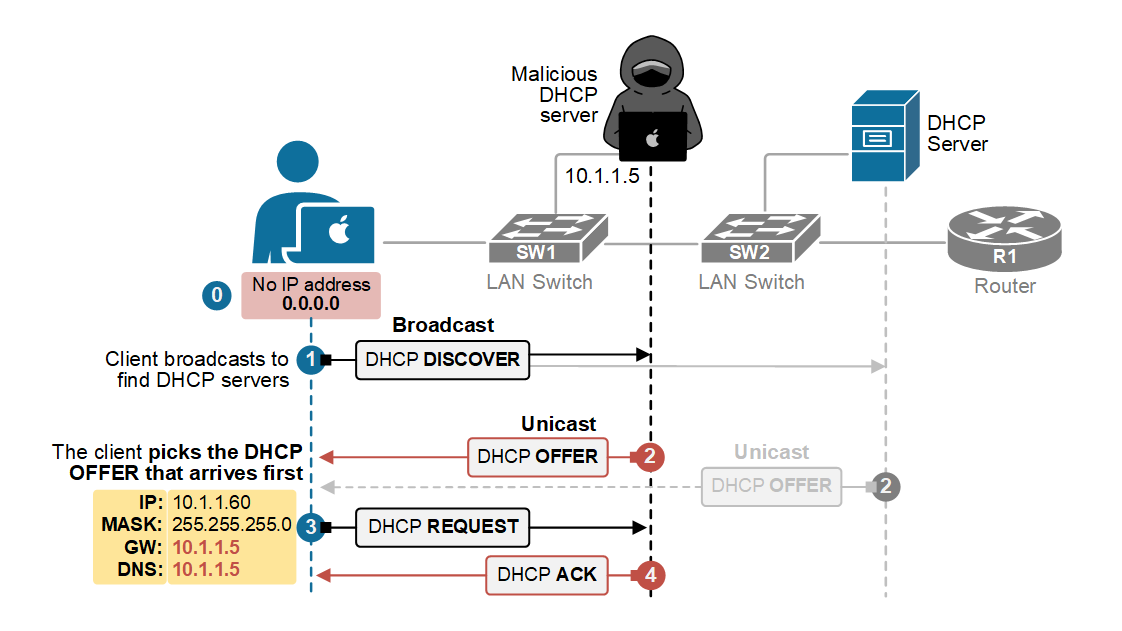
\includegraphics[width=0.4\textwidth]{../picts/dhcp-snooping.png}
\end{figure}

\paragraph{Mitigazione}
\begin{itemize}
    \item \textbf{DHCP Snooping}: configurabile sugli switch di livello 2, filtra i messaggi DHCP provenienti da porte non fidate (untrusted). Utilizza la DHCP Option 82.
\end{itemize}

\subsubsection{1.2 Protocolli di Intra-AS Routing (RIP e OSPF)}

\paragraph{RIP (Routing Information Protocol)}
\textbf{Funzionamento}
RIP è un protocollo di intra-routing di tipo \emph{Distance Vector} basato sul conteggio degli hop. I router vicini si scambiano periodicamente (ogni 30 secondi) messaggi di aggiornamento (\emph{RIP response message} o \emph{advertisements}) per informare della loro distanza da specifiche sottoreti (fino a 25 per messaggio). La tabella di routing di ogni nodo registra la sottorete di destinazione, il router vicino a cui inoltrare il pacchetto e il costo. I messaggi RIP utilizzano il protocollo UDP sulla porta 520.

\textbf{Vulnerabilità}
\begin{itemize}
    \item \textbf{Reflection DDoS}: (usando richieste IP spoofate per amplificare il traffico) o immissione di rotte fasulle per impersonare host o reindirizzare il traffico verso la macchina dell'attaccante.
\end{itemize}

\textbf{Mitigazione}
Restrizione dei pacchetti TCP/UDP 520 sui router di frontiera e Autenticazione (RIPv2 supporta MD5).

\paragraph{OSPF (Open Shortest Path First)}
\textbf{Funzionamento}
OSPF è un protocollo \emph{Link-State}. Invece di scambiarsi solo distanze tra vicini, ogni router distribuisce informazioni sullo stato dei propri collegamenti a tutti i router dell'AS tramite messaggi LSA (\emph{Link-State Advertisements}), inviati in caso di cambiamenti o periodicamente (ogni 30 minuti). 
Raccogliendo tutti gli LSA, ogni router costruisce internamente un'identica mappa topologica della rete e vi applica l'algoritmo di Dijkstra per calcolare l'albero dei percorsi minimi (\emph{shortest-path tree}) avendo se stesso come radice. I messaggi OSPF viaggiano direttamente incapsulati in IP (non usano TCP/UDP) e supportano l'autenticazione.

\textbf{Vulnerabilità}
Gli attacchi a OSPF possono sfruttare tecniche generiche come eavesdropping, message replay, message insertion/deletion/modification, Man-in-the-Middle e Denial-of-Service (DoS). 
Questi attacchi mirano a causare gravi danni all'infrastruttura, tra cui congestione di rete, partizionamento, \emph{black-holing} (soppressione del traffico), instabilità (churn e routing loop), o esaurimento delle risorse (overload di messaggi OSPF che saturano memoria e code del router).

\begin{itemize}
    \item \textbf{Max Age Attack}: L'attaccante inietta pacchetti LSA impostando il valore di età massima (3600 secondi, ovvero un'ora). Il router legittimo risponde generando un aggiornamento per contrastare l'anomalia, ma l'aggressore continua a inondare la rete con i pacchetti ``max age'', causando profonda instabilità e condizioni di DoS.
    \item \textbf{Sequence++ Attack}: L'attaccante inietta un LSA falso con un numero di sequenza incrementato, costringendo i nodi ad accettarlo come un aggiornamento più ``fresco''. Il router vittima tenta di ripristinare la rotta inviando un LSA con una sequenza ancora maggiore, innescando una continua sovrascrittura che destabilizza il routing globale.
    \item \textbf{Max Sequence Attack}: Viene iniettato un LSA malevolo con il numero di sequenza massimo consentito (\texttt{0x7FFFFFFF}). In molti casi, questo pacchetto estremo non viene eliminato dalle difese e persiste nel database per un'ora, garantendo all'attaccante il controllo prolungato del percorso.
    \item \textbf{Bogus LSA Attack}: Sfrutta specifiche vulnerabilità software (come i bug storici nel demone GateD) per forzare OSPF a ricalcolare le rotte alterando in modo malevolo i costi dei collegamenti. Questo permette di reindirizzare tutto il traffico verso un host controllato o provocare crash di sistema.
\end{itemize}

\textbf{Designated Router (DR) Attack}:
All'interno di reti condivise (come le LAN), OSPF elegge un Designated Router (DR) e un Backup DR (BDR) incaricati di inviare gli LSA di rete per conto degli altri nodi; tale elezione avviene tramite lo scambio di pacchetti \emph{Hello}. Un attaccante può alterare il processo in vari modi:
\begin{itemize}
    \item Falsificare i messaggi \emph{Hello} per eleggere il proprio router (o un ``phantom router'' inesistente) come DR/BDR.
    \item Declassare o spogliare del ruolo il DR autentico alterandone i pacchetti in transito.
\end{itemize}
Prendendo il controllo del ruolo di DR, l'attaccante manipola l'intera visione topologica degli altri nodi, potendo ad esempio isolare l'intera LAN o creare un massiccio \emph{black hole} in grado di intercettare e far cadere la maggior parte del traffico dell'Autonomous System.

\subsection{2. Attacchi al BGP (Border Gateway Protocol)}

\subsubsection{2.1 Introduzione a BGP}
Il BGP è il protocollo standard per l'inter-AS routing. 
BGP è un \emph{Path Vector protocol}: scambia informazioni di raggiungibilità delle sottoreti tenendo traccia dell'intero percorso (AS-PATH) per prevenire loop e applicare politiche di instradamento. 
Esistono eBGP (External BGP, tra AS diversi) e iBGP (Internal BGP, all'interno dello stesso AS).

\begin{figure}[h!]
    \centering
    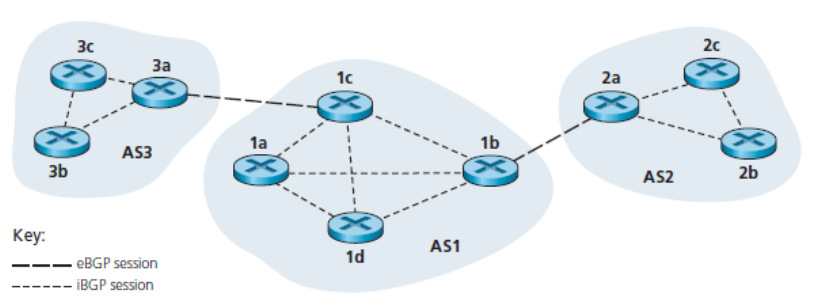
\includegraphics[width=0.4\textwidth]{../picts/ebg-ibgp.png}
\end{figure}

\subsubsection{2.2 Problemi di Sicurezza e Vulnerabilità}
BGP è stato progettato senza meccanismi nativi di autenticazione o integrità nei messaggi di Update. Questo permette a un attaccante di:
\begin{itemize}
    \item Falsificare rotte.
    \item Creare ``Blackhole'' per il traffico.
    \item Deviare il traffico per eavesdropping (intercettazione) o DDoS.
\end{itemize}

\paragraph{Tecniche di Attacco}
\begin{itemize}
    \item \textbf{Attacchi Denial of Service}: SYN flooding sui router BGP, invio di TCP RST per causare la caduta della sessione e instabilità (Route-flapping).
    \item \textbf{Prefix Hijacking (Dirottamento del Prefisso)}: un AS annuncia la paternità di un prefisso IP che non possiede. Il router diffonde l'annuncio e il traffico globale viene deviato verso l'AS attaccante.
    \item \textbf{De-aggregation (Traffic Attractor)}: sfruttando la regola per cui i router preferiscono il \emph{longest prefix match} (l'indirizzo più specifico), un AS malizioso può ``spezzare'' il blocco IP della vittima in blocchi più piccoli e annunciarli. Internet darà precedenza a queste rotte fasulle.
    \item \textbf{AS-Path Shortening}: un AS malevolo può rimuovere degli AS dal vettore per far apparire la propria rotta più breve e attrattiva, ingannando il meccanismo di selezione del miglior percorso.
\end{itemize}

\subsubsection{2.4 Difese e Mitigazioni}
Risolvere il problema del BGP è difficile per via dell'elevato numero di ISP decentralizzati. Le soluzioni attuali o proposte includono:
\begin{itemize}
    \item \textbf{Route Filtering}: gli ISP controllano mediante egress/ingress filter le rotte comunicate dai peer per verificare la correttezza del possesso degli IP rispetto agli Internet Routing Registries (IRRs).
    \item \textbf{BGP TTL Security Hack (RFC 3682)}: i messaggi eBGP vengono inviati con TTL 255. Il ricevente scarta i pacchetti con TTL inferiore a 254 (poiché i peer diretti sono a distanza di 1 hop), impedendo attacchi da nodi remoti.
    \item \textbf{MD5 Authentication (RFC 2385)}: estensione TCP che calcola un hash MD5 sull'header e payload, proteggendo la sessione da session hijacking e man-in-the-middle. Non usa IPsec direttamente ma agisce al livello TCP.
    \item \textbf{RPKI (Resource Public Key Infrastructure) e S-BGP}: meccanismi crittografici basati su Public Key Infrastructure. RPKI fornisce i ROA (Route Origin Authorizations) firmati dai RIR (es. RIPE, ARIN) per attestare l'appartenenza dei prefissi agli ASN. S-BGP (Secure BGP) aggiunge la firma crittografica degli attributi e dell'AS-PATH, benché la sua adozione globale sia frenata dai costi computazionali e dalla necessità di supporto generalizzato da tutti gli ISP.
\end{itemize}

\subsection{3. IPSEC e VPN}

\subsubsection{3.1 Introduzione allo Stack dei Protocolli e Problemi di Sicurezza}
Il protocollo IP di per sé è \emph{unreliable} e \emph{connectionless}, e non offre:
\begin{itemize}
    \item Autenticazione e integrità dei dati.
    \item Confidenzialità.
    \item Non-ripudio.
\end{itemize}

Problemi tipici includono il \emph{Source Spoofing} e i pacchetti \emph{Replay}. La protezione può avvenire a diversi livelli:
\begin{itemize}
    \item \textbf{Livello 1 e 2}: Protezione fisica, WEP, 802.1x (Access control basato su porta LAN).
    \item \textbf{Livello 3}: \textbf{IPsec} (Autenticazione mutua, Access control, Confidenzialità e Integrità dei dati).
    \item \textbf{Livello 4+}: SSL/TLS (Secure Sockets Layer / Transport Layer Security) over TCP.
\end{itemize}

\subsubsection{3.2 Architettura IPSEC}
IPsec è una suite di protocolli standardizzata progettata per proteggere le comunicazioni su reti IP mediante l'autenticazione e/o la crittografia di ogni pacchetto IP in una sessione di dati. Include:
\begin{itemize}
    \item \textbf{IKE (Internet Key Exchange)}: negozia i parametri di sicurezza e stabilisce le chiavi (usa UDP porta 500 per ISAKMP).
    \item \textbf{ESP (Encapsulating Security Payload)}: cifra, autentica e rende sicuri i dati.
    \item \textbf{AH (Authentication Header)}: fornisce autenticazione e integrità, ma non confidenzialità.
\end{itemize}

\begin{figure}[h!]
    \centering
    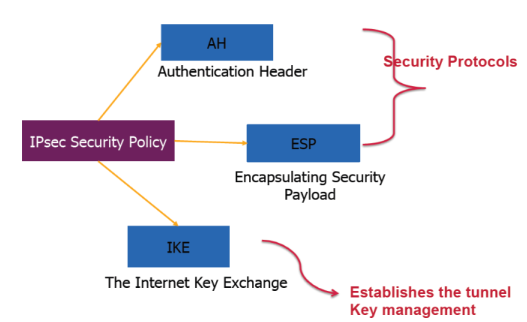
\includegraphics[width=0.4\textwidth]{../picts/ipsec-arch.png}
\end{figure}

\paragraph{Protocolli AH ed ESP}
\begin{itemize}
    \item \textbf{AH}: garantisce \textbf{autenticazione dell'origine} e \textbf{integrità dei dati}. Usa un Sequence Number a 32-bit contro gli attacchi replay ed algoritmi di hashing per la firma dei dati. Firmando anche l'header IP, AH è spesso incompatibile con NAT.
    \item \textbf{ESP}: aggiunge la \textbf{confidenzialità} (crittografia simmetrica) a quanto offerto da AH. In modalità Tunnel con ESP, l'intero pacchetto originale è cifrato, rendendo impossibile per un intermediario determinare gli indirizzi IP sorgente/destinazione originari.
\end{itemize}

\paragraph{Modalità di Funzionamento}
I protocolli base di IPsec (AH ed ESP) possono operare in due diverse modalità, influenzando come viene gestito l'header IP:
\begin{itemize}
    \item \textbf{Transport Mode}: Si utilizza tipicamente per comunicazioni end-to-end tra host (es. da client a server). In questo caso gli ``endpoint crittografici'' coincidono con gli ``endpoint di comunicazione''.
    \begin{itemize}
        \item \emph{AH in Transport Mode}: AH si inserisce tra l'header IP originale e il payload (es. TCP/UDP). Fornisce autenticazione dell'intero pacchetto (tranne i campi mutabili dell'header IP come il TTL).
        \item \emph{ESP in Transport Mode}: L'header ESP viene inserito dopo l'header IP originale e prima del payload. Il payload viene cifrato (e il trailer aggiunto), seguito dai dati di autenticazione ESP. L'header IP originale è lasciato in chiaro, permettendo l'instradamento nella rete.
    \end{itemize}
    \item \textbf{Tunnel Mode}: Si utilizza quando almeno un endpoint crittografico non è l'endpoint finale della comunicazione (tipico delle VPN site-to-site tra due gateway o router). Il pacchetto IP originale viene interamente incapsulato in un nuovo pacchetto IP.
    \begin{itemize}
        \item \emph{AH in Tunnel Mode}: L'intero datagramma IP originale (header e payload) è protetto e inserito in un nuovo pacchetto IP. AH autentica sia il vecchio pacchetto che le parti immutabili del nuovo header IP esterno.
        \item \emph{ESP in Tunnel Mode}: L'intero pacchetto IP originale è considerato payload, viene cifrato e racchiuso tra l'header e il trailer ESP. Un nuovo header IP in chiaro viene preposto per instradare il pacchetto nel tunnel. La vera destinazione (contenuta nell'IP header originale) non è accessibile a chi ispeziona il traffico intermedio.
    \end{itemize}
\end{itemize}

\begin{figure}[h!]
    \centering
    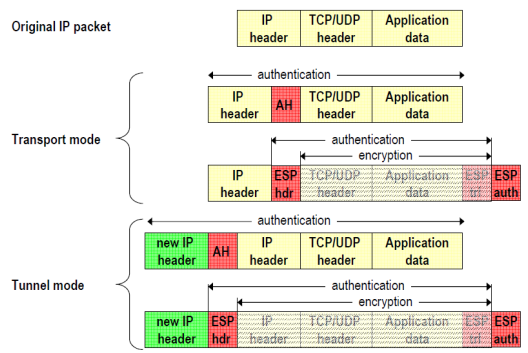
\includegraphics[width=0.4\textwidth]{../picts/ipsec-mode.png}
\end{figure}

\paragraph{Gestione delle Policy e Security Associations (SA, SADB, SPD)}
L'architettura IPsec utilizza tre componenti fondamentali per decidere come proteggere il traffico e mantenere lo stato delle connessioni sicure:
\begin{itemize}
    \item \textbf{SA (Security Association)}: È un concetto fondamentale in IPsec e definisce una collezione di attributi associati a una specifica connessione sicura. La SA è \textbf{unidirezionale} e \textbf{asimmetrica} (se ne richiedono almeno due per una comunicazione bidirezionale: una per il traffico in ingresso e una per quello in uscita). Una SA viene identificata univocamente da tre parametri:
    \begin{itemize}
        \item \emph{SPI (Security Parameter Index)}: un indice a 32 bit che svolge un ruolo simile ai numeri di porta nel TCP/UDP, indicando a quale SA appartiene il pacchetto entrante per processarlo correttamente.
        \item \emph{Indirizzo IP di destinazione}.
        \item \emph{Identificatore del protocollo di sicurezza} (AH o ESP).
    \end{itemize}
    \item \textbf{SPD (Security Policy Database)}: È il database che memorizza le politiche di sicurezza locali. Le politiche si basano sui selettori di traffico (IP locale, IP remoto, porte, protocolli come TCP/UDP). Per ogni flusso in rete, l'SPD forza una delle seguenti azioni:
    \begin{itemize}
        \item \emph{DISCARD}: il pacchetto viene scartato silenziosamente (es. regole di default deny per traffico intruso).
        \item \emph{BYPASS}: il pacchetto viene fatto passare in chiaro senza applicare IPsec (es. per consentire ICMP, o traffico HTTPS laddove l'amministratore voglia evitare di incapsulare una comunicazione già cifrata con TLS).
        \item \emph{PROTECT}: si richiede l'intervento di IPsec stabilendo o usando una SA esistente (es. forzare l'uso di ``ESP in Transport Mode con 3DES'' per le comunicazioni da un host a un server specifico).
    \end{itemize}
    \item \textbf{SADB (Security Association Database)}: È il database operativo che memorizza lo stato corrente di tutte le SA attive create tra i peer. Per ogni SA, il SADB contiene i parametri crittografici correnti negoziati (algoritmi, chiavi per la cifratura/autenticazione generate tramite IKE, durata della sessione e contatori dei Sequence Number).
\end{itemize}

\paragraph{Protezione Anti-Replay}
Sia i pacchetti protetti con AH che con ESP utilizzano un Sequence Number. 
Il mittente lo inizializza a zero quando stabilisce la SA e lo incrementa per ogni pacchetto trasmesso. Il ricevente esegue il controllo mantenendo una ``sliding window'' (finestra scorrevole, la cui dimensione minima pratica è di 32, o tipicamente 64 pacchetti).
\begin{itemize}
    \item Se un pacchetto arriva con un Sequence Number situato alla \emph{sinistra} della finestra (ovvero un valore vecchio), il ricevente lo rigetta considerandolo un potenziale Replay Attack.
    \item Se è all'interno della finestra (non ancora visto e con ICV valido) o alla \emph{destra} della finestra, il pacchetto è accettato e la finestra scorre di conseguenza.
\end{itemize}

\subsubsection{3.3 IKE (Internet Key Exchange)}
L'IKE fornisce un modo automatico per negoziare parametri e chiavi per IPsec. Si divide in due fasi:
\begin{itemize}
    \item \textbf{Fase 1}: crea un canale sicuro (ISAKMP SA) tra i peer. Opera in:
    \begin{itemize}
        \item \textbf{Main Mode}
        \begin{itemize}
            \item Tre scambi di informazioni tra i peers IPsec
            \item Iniziatore manda una o più proposte all'altro peer (responder)
            \item Il Responder seleziona una proposta
        \end{itemize}
        \item \textbf{Aggressive Mode} (più rapido ma meno sicuro, suscettibile a sniffing).
        \begin{itemize}
            \item Primo pacchetto mandato dall'iniziatore contiene tutte le info per stabilire una SA
            \item Il secondo pacchetto dal responder con tutti i parametri di sicurezza selezionati
            \item Il terzo pacchetto conclude l'autenticazione della sessione ISAKMP
        \end{itemize}
    \end{itemize}
    \item \textbf{Fase 2}: negozia le singole SA IPsec (unidirezionali) usate per il trasferimento dei dati, operando sul canale sicuro instaurato nella Fase 1.
\end{itemize}

\subsubsection{3.4 Virtual Private Network (VPN)}
Le VPN permettono di creare una rete privata sicura su una rete pubblica (Internet) eliminando il bisogno di costose linee dedicate.
\begin{itemize}
    \item \textbf{Trusted VPN}: il provider garantisce l'integrità del percorso (es. MPLS), ma non ci sono garanzie di cifratura contro le intrusioni.
    \item \textbf{Secure VPN}: usa crittografia (come IPsec o SSL/TLS) per proteggere i dati nel transito, comportandosi come un ``Tunnel''.
    \item \textbf{Hybrid VPN}: unione delle due precedenti.
\end{itemize}

\textbf{Tipologie Topologiche}:
\begin{itemize}
    \item \textbf{Intranet VPN}: collega sedi fisse aziendali.
    \item \textbf{Remote Access (RAS) VPN}: collega client remoti a un gateway aziendale.
    \item \textbf{Extranet VPN}: collega reti di partner limitando gli accessi mediante firewall.
\end{itemize}

\textbf{Protocolli VPN}:
Oltre a IPsec, esistono \textbf{L2TP} e \textbf{PPTP} (oggi ritenuti insicuri a causa di vulnerabilità nell'MS-CHAP v2 e interventi della NSA, come rivelato dai leak di Snowden), \textbf{SSTP} (proprietario Microsoft) e \textbf{OpenVPN} (basato su OpenSSL, altamente flessibile, utilizza UDP/TCP per by-passare la censura, sebbene richieda software di terze parti).


% -------------------------------------------------------------
% APPUNTI 4: WEB SECURITY
% -------------------------------------------------------------
\subsection{Architettura Web e Protocollo HTTP}
L'architettura di base del web si fonda sull'interazione continua tra il Browser (lato client), il Web Application Server e un Database.

Il server web riceve le richieste e restituisce codice scritto in linguaggi specifici, interpretati dal browser:
\begin{itemize}
    \item Il linguaggio HTML fornisce la struttura e i contenuti ipertestuali della pagina.
    \item I fogli di stile a cascata (CSS) hanno lo scopo di separare il contenuto dallo stile di presentazione visiva.
    \item JavaScript (noto anche come ECMAScript) è il linguaggio di scripting che permette l'esecuzione di codice dinamico all'interno della pagina web.
    \item I server HTTP, come Apache, possono interagire con le applicazioni web tramite interfacce specifiche come CGI, FastCGI o tramite moduli per l'esecuzione diretta di script basati su PHP, Python o ASP.
\end{itemize}

Il protocollo HTTP regola la comunicazione attraverso richieste inviate dal client e risposte restituite dal server.
\begin{itemize}
    \item La richiesta HTTP di tipo GET invia i dati al server allegandoli direttamente all'interno dell'URL.
    \item La richiesta HTTP di tipo POST inserisce i dati all'interno del campo dati (body) della richiesta stessa.
\end{itemize}

\subsection{Gestione dello Stato e Cookie}
Il server web è intrinsecamente ``senza stato'' (stateless), il che significa che non mantiene nativamente una connessione a lungo termine con il client.
\begin{itemize}
    \item I cookie HTTP vengono utilizzati per sopperire a questa mancanza salvando le informazioni direttamente sul lato client.
    \item Il browser memorizza questi cookie e li allega automaticamente a ogni richiesta successiva effettuata verso il server di destinazione.
    \item I cookie di sessione sono fondamentali per la sicurezza, poiché memorizzano un ID di sessione univoco (solitamente un numero casuale) creato dopo l'accesso dell'utente.
    \item Possedere l'ID di sessione equivale ad avere l'accesso garantito al sistema autenticato.
\end{itemize}
Esistono tuttavia problematiche legate al tracciamento e alla privacy.
\begin{itemize}
    \item I cookie di terze parti sono spesso utilizzati dalle reti pubblicitarie (Advertisement Network) per tracciare il comportamento degli utenti attraverso domini e siti differenti.
\end{itemize}

\subsection{JavaScript, Sandbox e Comunicazione Asincrona}
Il codice JavaScript viene eseguito all'interno del browser in un ambiente sandboxed.
\begin{itemize}
    \item Il codice JavaScript può accedere ai dati in-page (DOM), ai dati di navigazione del browser (come cookie e cronologia) e interfacciarsi con la rete.
    \item Non può tuttavia accedere direttamente al file system locale di sistema senza che l'utente conceda un'esplicita autorizzazione (ad esempio tramite la selezione manuale di un file).
\end{itemize}

Per la comunicazione di rete lato client, vengono adottati meccanismi asincroni come Ajax e WebSocket:
\begin{itemize}
    \item Ajax (Asynchronous JavaScript and XML) utilizza richieste HTTP standard in modalità half-duplex, dove il browser invia una richiesta e attende che il server risponda.
    \item Sulle comunicazioni Ajax interviene la politica della Stessa Origine (Same-Origin Policy), la quale blocca la lettura della risposta da parte del browser se la richiesta è diretta verso un dominio diverso, prevenendo compromissioni della privacy.
    \item Il meccanismo CORS (Condivisione delle Risorse tra Origini) consente di allentare questa restrizione rigorosa tramite una whitelist di origini fidate fornita direttamente dal server.
    \item WebSocket differisce offrendo una comunicazione di tipo full-duplex, permettendo a browser e server di inviare dati in modo bidirezionale e continuo.
    \item A differenza di Ajax, il browser non limita i dati provenienti da WebSocket tramite la Same-Origin Policy, demandando il controllo critico degli accessi e la verifica dell'origine direttamente al lato server.
\end{itemize}

\subsection{Cross-Site Request Forgery (CSRF)}
La falsificazione delle richieste tra siti (CSRF) è un attacco informatico che sfrutta l'automazione dei browser.
\begin{itemize}
    \item Il problema principale alla base del CSRF risiede nell'incapacità del server di distinguere autonomamente tra una richiesta legittima proveniente dal proprio sito (same-site) e una richiesta falsificata proveniente dall'esterno (cross-site).
    \item Questo accade perché il browser dell'utente, in buona fede, allega in modo automatico i cookie di sessione validi in entrambe le casistiche.
\end{itemize}

\begin{figure}[h!]
    \centering
    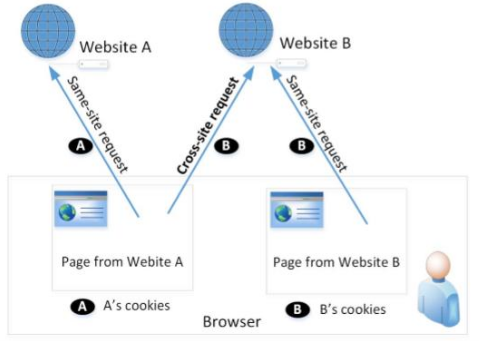
\includegraphics[width=0.4\textwidth]{../picts/csrf.png}
\end{figure}

Gli attacchi possono bersagliare diverse tipologie di richieste:
\begin{itemize}
    \item Negli attacchi CSRF su servizi HTTP GET, l'aggressore inserisce codice (come tag \texttt{<img>} o \texttt{<iframe>}) in una propria pagina malevola; appena la vittima la visita, il browser esegue una richiesta GET all'URL specificato, attivando l'azione sul sito bersaglio.
    \item Negli attacchi CSRF su servizi HTTP POST, l'aggressore può utilizzare script JavaScript nascosti all'interno della pagina per creare dinamicamente un modulo HTML (form) e forzarne l'invio automatico senza che l'utente debba cliccare alcun pulsante.
\end{itemize}

Esistono diverse contromisure tecniche per bloccare le vulnerabilità CSRF:
\begin{itemize}
    \item L'intestazione HTTP ``Referer'' identifica l'indirizzo della pagina di origine della richiesta, ma viene spesso rimossa dai client per preservare la cronologia e la privacy, rendendola una fonte inaffidabile per i server.
    \item L'attributo ``SameSite'' dei cookie (che può assumere i valori \emph{Strict} o \emph{Lax}) indica al browser di non inviare il cookie nel caso in cui venga rilevata una richiesta cross-site.
    \item L'implementazione di un token segreto casuale, generato dal server e inserito all'interno di ogni pagina web (spesso come campo nascosto nei form), garantisce sicurezza; l'attaccante non può leggerlo o indovinarlo a causa delle limitazioni imposte dalla Same-Origin Policy.
\end{itemize}

\subsection{Cross-Site Scripting (XSS)}
Il Cross-Site Scripting è una vulnerabilità che si verifica quando un'applicazione web esegue nel browser della vittima uno script malevolo iniettato da un aggressore esterno.
\begin{itemize}
    \item Poiché il codice JavaScript sembra provenire dal sito web originale, il browser lo considera attendibile e gli concede i medesimi privilegi del sito.
    \item Il codice malevolo può alterare il contenuto del DOM, inviare richieste di spoofing per conto dell'utente, e rubare dati sensibili privati come i cookie di sessione.
\end{itemize}

Esistono due macro-categorie principali per l'esecuzione di attacchi XSS:
\begin{itemize}
    \item \textbf{Attacco XSS non persistente (riflesso)}: Se il server web accetta input non filtrati e li rimanda (riflette) indietro all'utente, un aggressore può nascondere il codice JavaScript in un link generato ad hoc; quando la vittima ci clicca sopra, la pagina restituita includerà il codice eseguibile.
    \item \textbf{Attacco XSS persistente (memorizzato)}: L'aggressore invia il proprio payload malevolo a un sito web in modo che venga archiviato permanentemente (ad esempio all'interno di un commento o di un profilo utente); chiunque visualizzi successivamente quel contenuto eseguirà il codice sul proprio dispositivo.
\end{itemize}

Gli attacchi XSS persistenti possono essere utilizzati per creare un worm XSS:
\begin{itemize}
    \item Sfruttando le API del DOM, un worm JavaScript può accedere al proprio nodo interno per ottenere una copia del proprio codice sorgente.
    \item In alternativa, tramite l'approccio di collegamento, il codice JavaScript può essere incluso nella pagina infetta includendo l'attributo \texttt{src} rivolto verso il server dell'attaccante.
    \item Ogni volta che il profilo infetto viene visitato da una nuova vittima, il codice malevolo modifica dinamicamente il profilo del visitatore iniettando una copia del worm e garantendone l'espansione esponenziale.
\end{itemize}

Per mitigare efficacemente il rischio associato agli attacchi XSS, i sistemi adottano approcci di difesa standardizzati:
\begin{itemize}
    \item Filtri per codice JavaScript potenzialmente pericoloso (es. tag \texttt{<script>}) sugli input dell'utente utilizzando librerie specifiche.
    \item La codifica di markup HTML come entità sicure prima di renderizzarli sulla pagina, forzando i browser a visualizzarli come semplice testo stringa senza eseguirli.
    \item La Content Security Policy (CSP) è un'intestazione di sicurezza che sconfigge l'XSS vietando categoricamente l'esecuzione di script in linea (inline) e obbligando la definizione di una rigida whitelist di origini permesse o l'adozione di ``nonce'' crittografici autorizzati.
\end{itemize}

\end{document}
